\documentclass{article}
\usepackage[utf8]{inputenc} %кодировка
\usepackage[T2A]{fontenc}
\usepackage[english,russian]{babel} %русификатор 
\usepackage{mathtools} %библиотека матеши
\usepackage[left=1cm,right=1cm,top=2cm,bottom=2cm,bindingoffset=0cm]{geometry} %изменение отступов на листе
\usepackage{amsmath}
\usepackage{graphicx} %библиотека для графики и картинок
\graphicspath{}
\DeclareGraphicsExtensions{.pdf,.png,.jpg}
\usepackage{subcaption}
\usepackage{pgfplots}

\begin{document}

\thispagestyle{empty}
% НАЧАЛО ТИТУЛЬНОГО ЛИСТА
\begin{center}
        \Large
        Федеральное государственное автономное \\
        образовательное учреждение высшего образования \\ 
        «Научно-образовательная корпорация ИТМО»\\
        \vspace{0.5cm}
        \large
        Факультет программной инженерии и компьютерной техники \\
        Направление подготовки 09.03.04 Программная инженерия \\
        \vspace{1cm}
        \Large
        \textbf{Отчёт по расчетно-графической работе №4} \\
        По дисциплине «Математический анализ» (второй семестр)\\
        \large
        \vspace{8cm}
    
        \begin{minipage}{.33\textwidth}
        \end{minipage}
        \hfill
        \begin{minipage}{.4\textwidth}
            \textbf{Группа}: \vspace{.1cm} \\
            \ МАТБАЗ 1.5\\ \\
            \textbf{Студенты}: \vspace{.1cm} \\
            \ Андриянова Софья\\
            \ Беляев Михаил\\
            \ Билошицкий Михаил\\
            \ Дениченко Александр\\
            \ Разинкин Александр\\ \\
            \textbf{Лектор}: \vspace{.1cm} \\
            \ Правдин Константин Владимирович \\ \\
            \textbf{Практик}:  \\
            \ Правдин Константин Владимирович
        \end{minipage}
        \vfill
    Санкт-Петербург\\ 2023 г.
    \end{center}
 
% КОНЕЦ ТИТУЛЬНОГО ЛИСТА

\newpage


% задание 1 начало
\section{Ряд Тейлора}
а)


\textbf{Задание:} Некоторую функцию разложили в ряд Маклорена и, придав аргументу x определённое
значение, получили данный числовой ряд. Найдите его сумму.\\
\begin{equation*}
    \sum_{n = 1}^{\infty} \frac{(-1)^{n-1}}{\sqrt{3^n}(2n-1)}
\end{equation*}


\textbf{Решение:}\\
Перейдём к функциональному ряду, где агрумент возьмём за x.\\
\begin{equation*}
     x = \frac{1}{\sqrt[4]{3}}
\end{equation*}
Имеем:
\begin{equation*}
    \sum_{n = 1}^{\infty} \frac{(-1)^{n-1}x^{2n}}{(2n-1)}=x\cdot \sum_{n = 1}^{\infty}\frac{(-1)^{n-1}x^{2n-1}}{(2n-1)}
\end{equation*}
Заметим, что формула $a_n$ очень похожа на формулу $\widetilde{a_n}$ при стандартном разложении в ряд Маклорена функции $arctg\ x$\\
\begin{equation*}
    x\cdot \sum_{n = 1}^{\infty}\frac{(-1)^{n-1}x^{2n-1}}{(2n-1)}=arctg(x)\cdot x;
\end{equation*}
Данное разложение справедливо только при $\forall x\in[-1;1]$\\
Сделаем обратную замену, где $x=\frac{1}{\sqrt[4]{3}}\Longrightarrow \underline{ S=\frac{arctg(\frac{1}{\sqrt[4]{3}})}{\sqrt[4]{3}}}$ (сумма ряда)
\\ \\б)


\textbf{Задание:} Найдите первообразную данной функции в виде ряда, используя стандартные разложения
степенных рядов, а также свойства их сложения и умножения.
\begin{equation*}
    f(x)=\frac{sinx}{x}
\end{equation*}


\textbf{Решение:}\\
Разложим функцию $sin(x)$, применяя стандартные разложения в ряд Маклорена:\\
\begin{equation*}
    sin(x)=\sum_{n = 1}^{\infty} (-1)^{n+1}\frac{x^{2n-1}}{(2n-1)!}
\end{equation*}
Теперь мы можем разделить ряд на x и предствить функцию в виде $f(x)=(F(x))'$
\begin{equation*}
   \frac{sin(x)}{x} = \sum_{n = 1}^{\infty} (-1)^{n+1}\frac{x^{2n-2}}{(2n-1)!} =\sum_{n = 1}^{\infty} \left((-1)^{n+1}\frac{x^{2n-1}}{(2n-1)!(2n-1)}\right)'=^?\left(\sum_{n = 1}^{\infty} (-1)^{n+1}\frac{x^{2n-1}}{(2n-1)!(2n-1)}\right)'
\end{equation*}
Для равносильного перехода от суммы производных к производной суммы нам потребудется доказать, что ряд, который образует сумма, сходится равномерно. Для этого подберём мажорирующий ряд, который будет работать в определённой области:\\
\begin{equation*}
    \frac{|x^{2n-1}|}{(2n-1)!(2n-1)}\leq  \frac{1}{(2n-1)!(2n-1)}
\end{equation*}
Докажем сходимость мажорирующего ряда по признаку Даламбера:
\begin{equation*}
    \lim_{n\rightarrow \infty }\frac{(2n-1)!(2n-1)}{(2(n+1)-1)!(2(n+1)-1)} = \lim_{n\rightarrow \infty }\frac{(2n-1)!(2n-1)}{(2n+1)!(2n+1)}=\lim_{n\rightarrow \infty }\frac{(2n-1)}{2n(2n+1)^2}=0\Rightarrow CX
\end{equation*}
Из сходимости мажорирующего ряда следует равномерная и абсолютная сходимость изначального ряда, а это значит, что мы можем перейти от суммы производных к производной суммы.
\begin{equation*}
    (F(x))'=\left(\sum_{n = 1}^{\infty}(-1)^{n+1}\frac{x^{2n-1}}{(2n-1)!(2n-1)}+C\right)'
\end{equation*}
\begin{equation*}
    \underline{ F(x)=\sum_{n = 1}^{\infty}(-1)^{n+1}\frac{x^{2n-1}}{(2n-1)!(2n-1)}+C}
\end{equation*}
\\ \\в)


\textbf{Задание:} Найдите первые k членов разложения в степенной ряд решения дифференциального
уравнения при указанных начальных условиях. Изобразите на графике.
\begin{equation*}
    y'=\frac{x}{\sqrt{y}}+2,\ y(0)=1,\ k=5
\end{equation*}


\textbf{Решение:}\\
Для разложения в ряд Маклорена воспользуемся формулой:
\begin{equation*}
    y=\sum_{n = 0}^{\infty}  \frac{f^{(n)}(x_0)}{n!}\cdot(x-x_0)^n
\end{equation*}
Первый член разложения в ряд Маклорена:\\
\[
    y(0)=1\]\\
Производная для второго члена член разложения в ряд Маклорена:\\
\[
    y'=\frac{x}{\sqrt{y}}+2
\]
\[
    y'(0)=2\]\\
Производная для тертьего члена разложения в ряд Маклорена:\\
\[
    y''=(\frac{x}{\sqrt{y}}+2)'=\frac{\sqrt{y}+x(\sqrt{y})'}{y}=\frac{\sqrt{y}+x\cdot \frac{1}{2\sqrt{y}}\cdot y'}{y}
\]
\[
    y''(0)=\frac{1}{1}=1
\]
\\
Производная для четвёртого члена разложения в ряд Маклорена:\\
\[
    y'''=\frac{\frac{2\sqrt{y}y'+2\sqrt{y}xy''-\frac{xy'}{\sqrt{y}}}{4y}}{y}- \frac{y'\cdot\frac{2\sqrt{y}y'+2\sqrt{y}xy''-\frac{xy'}{\sqrt{y}}}{4y}}{y^2}
\]
\[
    y'''(0)=-\frac{5}{4}
\]
\\
Производная для пятого члена разложения в ряд Маклорена:\\
\[
    y^{IV}=\frac{\left(\frac{y^{'2}}{\sqrt{y}}+\sqrt{y}y''+\frac{xy'y''}{\sqrt{y}}+2\sqrt{y}y''+2\sqrt{y}xy'''-\frac{\sqrt{y}y'^2+\sqrt{y}x2y'y''-\frac{xy'^3}{2\sqrt{y}}}{y}\right)4y^2-\left(2\sqrt{y}y'+2\sqrt{y}xy''-\frac{xy'^2}{\sqrt{y}}\right)8yy'}{16y^4}-
\]
\[
    -\frac{\left(\frac{y^{'2}}{\sqrt{y}}+4\sqrt{y}y''y'''+\frac{y'^2xy'}{\sqrt{y}}+2\sqrt{y}y''y'+2\sqrt{y}y'y'''+2\sqrt{y}y''^2-\frac{\sqrt{y}y'^3+3\sqrt{y}xy'^2y''-\frac{xy'^4}{2\sqrt{y}}}{y}\right)4y^3-\left(2\sqrt{y}y'^2+2\sqrt{y}xy''y'-\frac{xy'^3}{\sqrt{y}}\right)12y^2y'}{16y^9}
\]
\[
    y^{IV}(0)=\frac{15}{2}
\]
Ряд будет выглядеть следующим образом:\\
\[
    f(x) = 1 +\frac{2}{1!}x+\frac{1}{2!}x^2+\frac{-\frac{5}{4}}{3!}x^3+\frac{\frac{15}{2}}{4!}x^4
\]
Покажем на графике:\\
\begin{center}
    \begin{tikzpicture}
        \begin{axis}[
        axis lines = middle,
        xlabel = $x$,
        ylabel = $f(x)$,
        xmin = -5,
        xmax = 5,
        ymin = -5,
        ymax = 5,
        legend pos = north west,
        legend style={anchor=north west, xshift=-3cm, yshift=-6cm} % Сдвиг рамки с подписью влево и вниз на 0.5 см
        ]
        \addplot [
        domain=-5:5,
        samples=100,
        color=blue,
        ]
        {1 + 2*x + (1/2)*x^2 - (5/4)*(1/6)*x^3 + (15/2)*(1/24)*x^4};
        \addlegendentry{$f(x)=1 +\frac{2}{1!}x+\frac{1}{2!}x^2+\frac{-\frac{5}{4}}{3!}x^3+\frac{\frac{15}{2}}{4!}x^4$}
        \end{axis}

        \end{tikzpicture}
        \captionof{figure}{Вспомогательные построения}
\end{center}
\section{Ряд Фурье}


\textbf{Задание:} С помощью разложения в ряд Фурье данной функции в интервале $(-\pi;\pi)$ найдите сумму
указанного числового ряда.\\
\[
    f(x)=|x|,\ \sum_{n=1}^{\infty}\frac{1}{(2n-1)^2}
\]
\textbf{Решение:}\\


1)Представим функцию её рядом Фурье.\\
\begin{center}
    \begin{tikzpicture}
        \begin{axis}[
            axis lines = middle,
            xlabel = \(x\),
            ylabel = \(f(x)\),
            xmin = -5,
            xmax = 5,
            ymin = 0,
            ymax = 5,
            extra x ticks = {-3.14159, 3.14159},
    extra x tick labels = {\(-\pi\), \(\pi\)},
        ]
        \addplot [
            domain=-5:5,
            samples=100,
            color=blue,
        ]
        {abs(x)};
        \draw[dashed] (axis cs:3.14159, 0) -- (axis cs:3.14159, 5);
        \draw[dashed] (axis cs:-3.14159, 0) -- (axis cs:-3.14159, 5);
        \addplot [
            mark = *,
            mark options = {color = red},
            only marks,
        ] 
        coordinates { (3.14159, 0) };
        \addplot [
            mark = *,
            mark options = {color = red},
            only marks,
        ] 
        coordinates { (-3.14159, 0) };
        \end{axis}
        \end{tikzpicture}
        \captionof{figure}{Функция данная по условию}
\end{center}


Если мы рассматриваем фиксированный отрезок \([- \pi, \pi]\), то коэффициенты ряда Фурье для тригонометрической формы могут быть вычислены следующим образом:

\[a_0 = \frac{1}{\pi} \int_{-\pi}^{\pi} f(x) dx\]
\[a_n = \frac{1}{\pi} \int_{-\pi}^{\pi} f(x) \cos(n x) dx\]
\[b_n = \frac{1}{\pi} \int_{-\pi}^{\pi} f(x) \sin(n x) dx\]

где:
- \(f(x)\) - функция, определенная на отрезке \([- \pi, \pi]\)
- \(n\) - порядок гармоники
- \(a_0\) - коэффициент постоянной составляющей (среднее значение функции \(f(x)\) на отрезке \([- \pi, \pi]\))
- \(a_n\) - коэффициенты косинусной гармоники
- \(b_n\) - коэффициенты синусной гармоники

Полученные коэффициенты могут быть использованы для записи ряда Фурье в виде:

\[f(x) = \frac{a_0}{2} + \sum_{n=1}^{\infty} \left[ a_n \cos(n x) + b_n \sin(n x) \right]\]

В данном случае, ряд Фурье представляет функцию \(f(x)\) в виде суммы косинусов и синусов с различными частотами, где каждый член в сумме соответствует гармонике с определенной частотой и амплитудой.
Заметим, что функция является чётной, а значит элемент $b_n$ будет равен нулю по одному из свойств ряда Фурье, а также мы будем рассматривать удвоенные интегралы по промежутку $(0;\pi)$.\\


\[a_0 = \frac{1}{\pi} \int_{-\pi}^{\pi} |x| dx= \frac{2}{\pi}\int_{0}^{\pi}xdx=\frac{2}{2\pi}x^2|_0^{\pi}=\pi
\]
\[a_n = \frac{1}{\pi} \int_{-\pi}^{\pi} |x| \cos(n x) dx= \frac{2}{\pi} \int_{-\pi}^{\pi} x \cos(n x) dx= \frac{2}{\pi n} \int_{-\pi}^{\pi} x d(\sin(n x))=\frac{2}{\pi n}\left(x\cdot sin(nx)|_0^{\pi}-\int_{0}^{\pi}sin(nx)dx\right)=
\]
\[
    =\frac{2}{\pi n}\left(0-\frac{1}{n}\int_{0}^{\pi}sin(nx)d(nx)\right)=\frac{2}{\pi n^2}(-1)^n-\frac{2}{\pi n^2}=\frac{2}{\pi n^2}((-1)^n-1)
\]
Представим разложенную функцию:
\[
    y=|x|=\frac{\pi}{2}+\sum_{n=1}^{\infty}\frac{2}{\pi n^2}((-1)^n-1)cos(nx)=\left|n=0, 2, 4, ... \sum = 0;\ n=1, 3, 5, ... \sum = -2\right|=
\]
\[
    = \frac{\pi}{2}+\sum_{k=1}^{\infty}\frac{2}{\pi (2k-1)^2}\cdot(-2)\cdot cos((2k-1)x)=\frac{\pi}{2}-\sum_{k=1}^{\infty}\frac{4\cdot cos((2k-1)x)}{\pi(2k-1)^2}
\]
Положим, что $x=0$, тогда:
\[
    y(0)=\frac{\pi}{2}-\frac{4}{\pi}\sum_{k=1}^{\infty}\frac{1}{(2k-1)^2}
\]
Сравним с числовым рядом:
\[
    \sum_{k=1}^{\infty}\frac{1}{(2k-1)^2}=\left(\frac{\pi}{2}-y(0)\right)\cdot \frac{\pi}{4}
\]
Так как при $x=0\ f(0)=|0|$, тогда:\\
\[
    \sum_{k=1}^{\infty}\frac{1}{(2k-1)^2}=\left(\frac{\pi}{2}-y(0)\right)\cdot \frac{\pi}{4}= \frac{\pi^2}{8}
\]
Покажем в системе координат функцию и её разложение в ряд Фурье:\\
\begin{center}
    \begin{tikzpicture}
        \begin{axis}[
            axis lines = middle,
            xlabel = \(x\),
            ylabel = \(f(x)\),
            xmin = -5,
            xmax = 5,
            ymin = 0,
            ymax = 5,
            extra x ticks = {-3.14159, 3.14159},
    extra x tick labels = {\(-\pi\), \(\pi\)},
    legend style={anchor=north west, xshift=-9cm, yshift=-6.5cm} % Сдвиг рамки с подписью влево и вниз на 0.5 см
        ]
        \addplot [
            domain=-5:5,
            samples=100,
            color=green,
        ]
        {abs(x)};
        \addlegendentry{\(f(x) = |x|\)};
        \draw[dashed] (axis cs:3.14159, 0) -- (axis cs:3.14159, 5);
        \draw[dashed] (axis cs:-3.14159, 0) -- (axis cs:-3.14159, 5);
        \addplot [
            mark = *,
            mark options = {color = red},
            only marks,
        ] 
        coordinates { (3.14159, 0) };
        \addplot [
            mark = *,
            mark options = {color = red},
            only marks,
        ] 
        coordinates { (-3.14159, 0) };
        \addplot [
    color=blue,
] gnuplot {pi/2 + sum [n=1:3] 2/(pi * n^2) * ((-1)**n-1) * cos(n*x)};
\addlegendentry{\((-\pi;0)\)}
\addlegendentry{\((0;\pi)\)}
\addlegendentry{\(f(x) = \frac{\pi}{2} + \sum_{k=1}^{\infty} \frac{2}{\pi (2k-1)^2} \cdot (-2) \cdot \cos((2k-1)x)\)}
        \end{axis}
        \end{tikzpicture}
        \captionof{figure}{Разложение до k=3}
\end{center}
\section{Приближение ряда Фурье конечной суммой}
\textbf{Задание:}
В трёх однотипных опытах радиолюбителей на вход цифро-аналогового преобразователя
(ЦАП) был подан короткий цифровой сигнал формы, изображённой на рисунке.

\textbf{Решение:}\\
1)
\begin{center}
    \begin{tikzpicture}
    \begin{axis}[
        axis lines = middle,
        xlabel = \(x\),
        ylabel = \(y\),
        xmin = 0,
        xmax = 4,
        ymin = -1,
        ymax = 3,
        xtick = {0,1,2,3,4},
        ytick = {-1,0,1,2,3},
        xticklabels = {0,1,2,3,4},
        yticklabels = {-1,0,1,2,3},
    ]
    
    \addplot [
        domain=0:1,
        color=blue,
    ] {0};
    
    \addplot [
        domain=1:2,
        color=blue,
    ] {1};
    
    \addplot [
        domain=2:3,
        color=blue,
    ] {2};
    
    \addplot [
        domain=3:4,
        color=blue,
    ] {0};
    
    \end{axis}
    \end{tikzpicture}
    \captionof{figure}{Исходный график}
\end{center} 
Выпишем функцию, заданную кусочно:\\
\begin{equation*}
    f(x)=
    \begin{cases}
        0, x \in [0;1) \cup [3;4)\\
        1, x \in [1;2)\\
        2, x \in [2;3)
    \end{cases},\ T=4\ =>\ l=2
\end{equation*} 
Вычислим коэффиценты для разложения в ряд Фурье
\[
    a_0=\frac{1}{2}\int_{0}^{4}f(x)dx = \frac{1}{2}(\int_{0}^{1}0dx+\int_{1}^{2}1dx+\int_{2}^{3}2dx+\int_{3}^{4}0dx)=\frac{3}{2}
\]
\[
    a_n = \frac{1}{2}\int_{0}^{4}f(x)cos\left(\frac{\pi}{2}nx\right)dx=\frac{1}{2}\left(\int_{0}^{1}0cos\left(\frac{\pi nx}{2}\right)+\int_{1}^{2}1cos\left(\frac{\pi nx}{2}\right)+ \int_{2}^{3}2cos\left(\frac{\pi nx}{2}\right)+ \int_{3}^{4}0cos\left(\frac{\pi nx}{2}\right)\right)=
\]
\[=\frac{1}{2} \left(\int_{1}^{2} \cos\left(\frac{\pi nx}{2}\right) \, dx + \int_{2}^{3} 2 \cos\left(\frac{\pi nx}{2}\right) \, dx\right)= \left(\frac{2}{\pi n}sin(\frac{3\pi}{2} n)-\frac{1}{\pi n}sin\left(\frac{\pi}{2}n\right)-\frac{1}{\pi n}sin\left(\pi n\right)\right)\]


\[
    b_n = \frac{1}{2}\int_{0}^{4}f(x)sin\left(\frac{\pi}{2}nx\right)dx=\frac{1}{2}\left(\int_{0}^{1}0sin\left(\frac{\pi nx}{2}\right)+\int_{1}^{2}1sin\left(\frac{\pi nx}{2}\right)+ \int_{2}^{3}2sin\left(\frac{\pi nx}{2}\right)+ \int_{3}^{4}0sin\left(\frac{\pi nx}{2}\right)\right)=
\]
\[=\frac{1}{2} \left(\int_{1}^{2} \sin\left(\frac{\pi nx}{2}\right) \, dx + \int_{2}^{3} 2 \sin\left(\frac{\pi nx}{2}\right) \, dx\right)=\left(\frac{1}{\pi n}cos(\pi n)+\frac{1}{\pi n}cos\left(\frac{\pi}{2}n\right)-\frac{2}{\pi n}cos\left(\frac{3\pi}{2}n\right)\right)\]
Представим разложенную функцию:
\[
    f(x)= y=\frac{3}{4}+\sum_{n=1}^{k}(\left(-\frac{1}{\pi n}\sin\pi n-\frac{1}{\pi n}\sin\left(\frac{\pi}{2}n\right)+\frac{2}{n\pi}\sin\left(\frac{3\pi}{2}n\right)\right)\cos\frac{nx\pi}{2}+
\]
\[
    +\left(\frac{1}{\pi n}\cos\pi n+\frac{1}{\pi n}\cos\left(\frac{\pi}{2}n\right)-\frac{2}{\pi n}\cos\left(\frac{3\pi}{2}n\right)\right)\sin\left(\frac{nx\pi}{2}\right))\
\]
Графики опытов:
\begin{center}
    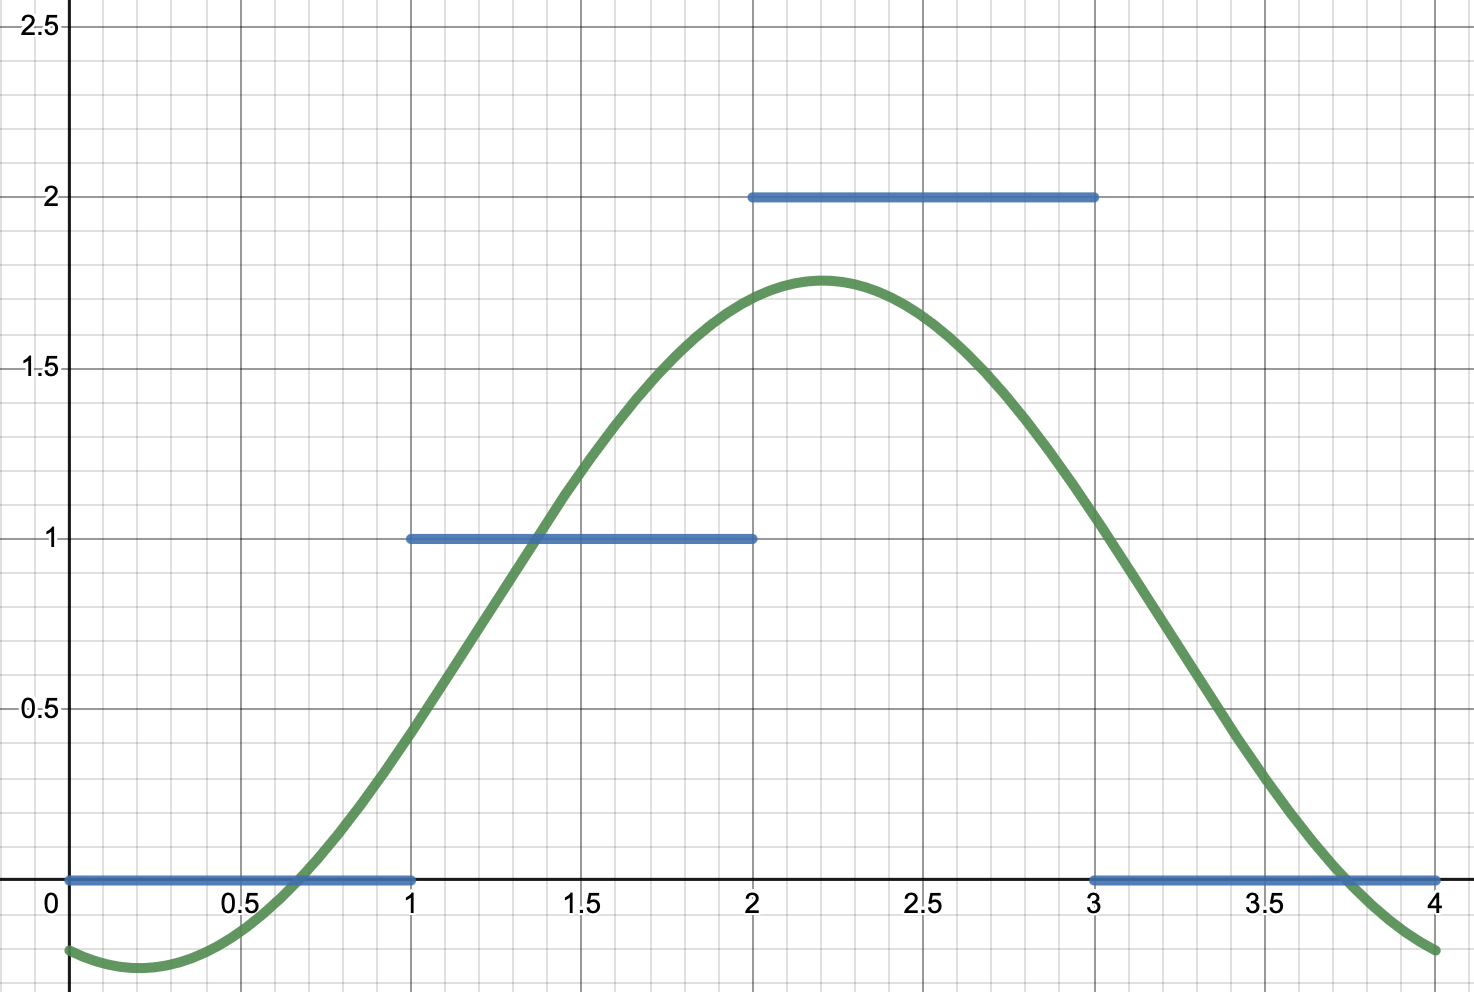
\includegraphics[width=.6\textwidth]{1}
    \captionof{figure}{Опыт первый}
\end{center} 
Максимальная ошибка ЦАП - 1.062
\begin{center}
    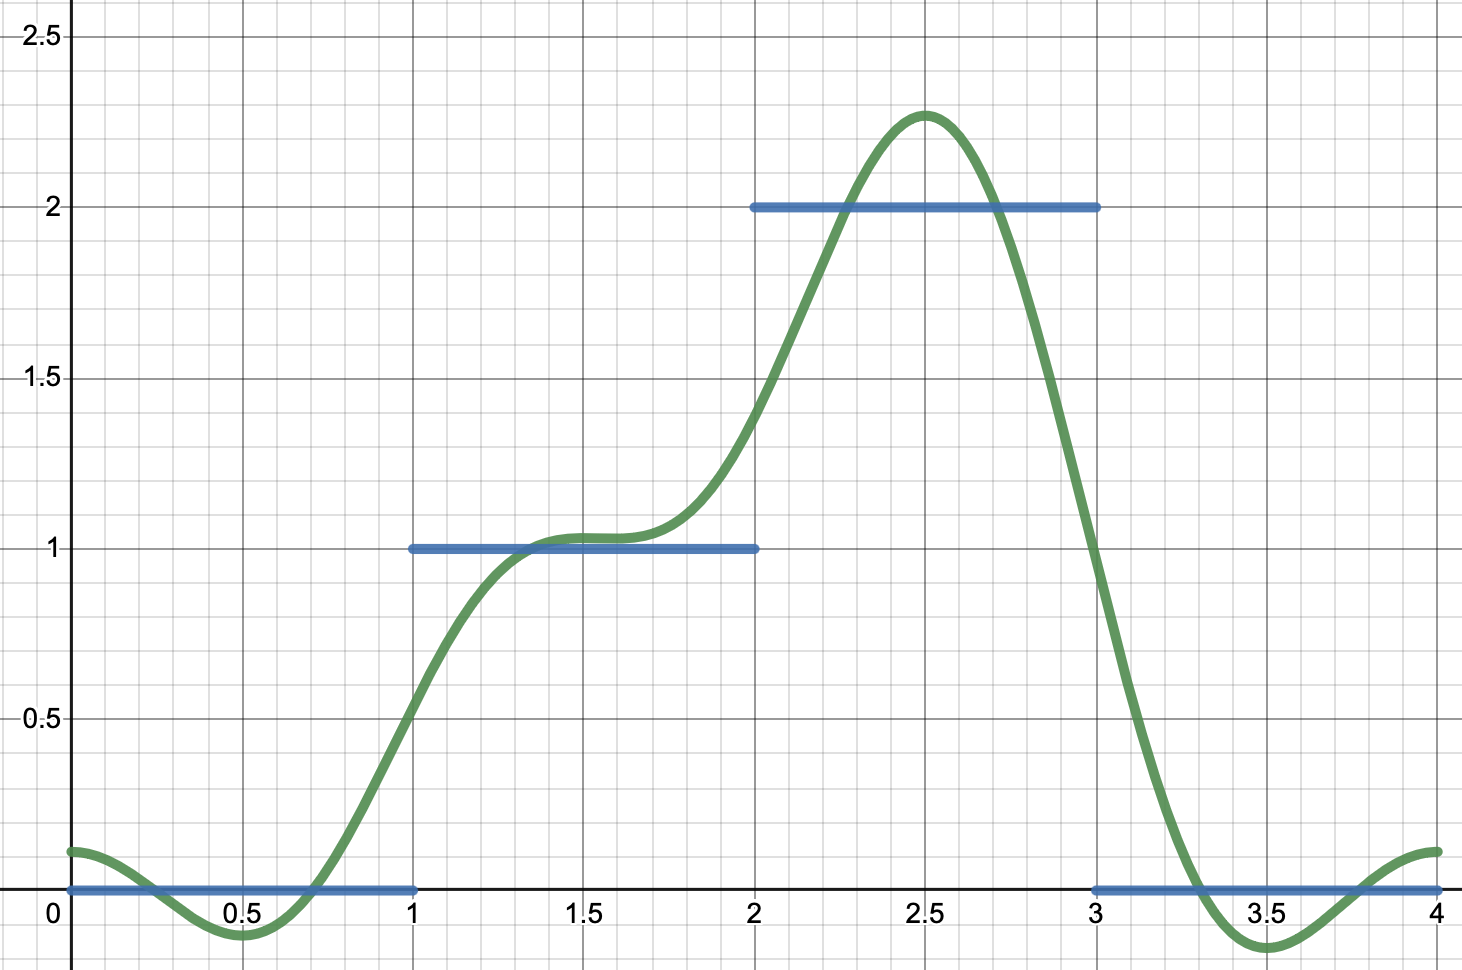
\includegraphics[width=.6\textwidth]{2}
    \captionof{figure}{Опыт второй}
\end{center} 
Максимальная ошибка ЦАП - 1.04
\begin{center}
    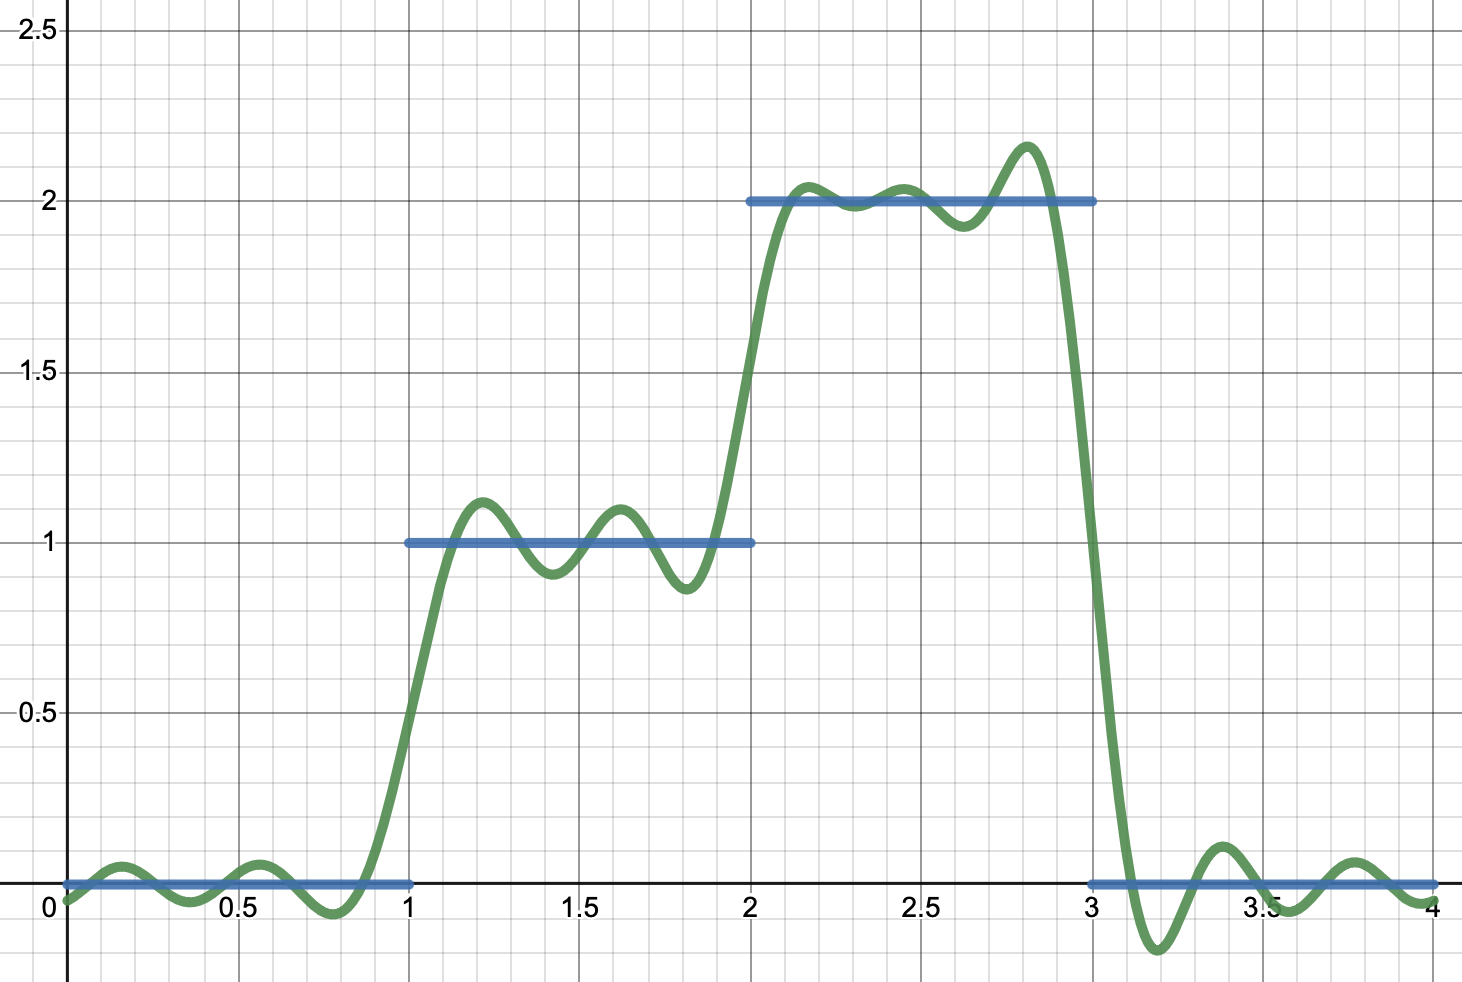
\includegraphics[width=.6\textwidth]{3}
    \captionof{figure}{Опыт третий}
\end{center}
Максимальная ошибка ЦАП - 1.0105


При росте гармоники, ошибка ЦАП уменьшается.


\end{document}